\documentclass[11pt]{article}
\usepackage{lastpage, fancyhdr,color,amsmath,amssymb,amsfonts,amscd, graphicx,latexsym,multirow}
\usepackage{makecell}
\usepackage{lipsum}
\usepackage{eurosym}
\usepackage[all]{xy}
\pagestyle{empty}
\usepackage[utf8]{inputenc}
\usepackage[T1]{fontenc}
\setlength\voffset{-1in}
\setlength\hoffset{-1in}
\setlength\topmargin{3cm}
\setlength\oddsidemargin{2.5cm}
\setlength\textheight{8in}
\setlength\textwidth{6.51in}\setlength\footskip{1in}
\setlength\headheight{12pt}
\setlength\headsep{0.06in}
\usepackage{caption, subcaption, amsfonts}
\usepackage{setspace}
\usepackage{epstopdf,sectsty}
\usepackage{relsize}
\usepackage{pgf, float}
\usepackage{url}
\usepackage{natbib}
\usepackage{csquotes}
\usepackage{wrapfig}

\definecolor{light-gray}{gray}{0.55}

\renewcommand{\contentsname}{Contenuti}
\renewcommand{\listfigurename}{Figure}

\title{Moto in un fluido denso}

\begin{document}
\pagestyle{fancy}
   \lhead{}\rhead{}
   \lfoot{\textcolor{light-gray}{\small Moto in un fluido denso}}
        \cfoot{{\thepage}}
        \rfoot{}
  \renewcommand{\headrulewidth}{0pt}




\newpage
\phantom{22}
\vspace{-3cm}

\begin{center}
% Logo copyright belongs to TUBITAK
% downloaded from https://www.tubitak.gov.tr/sites/default/files/tubitak_logo.jpg
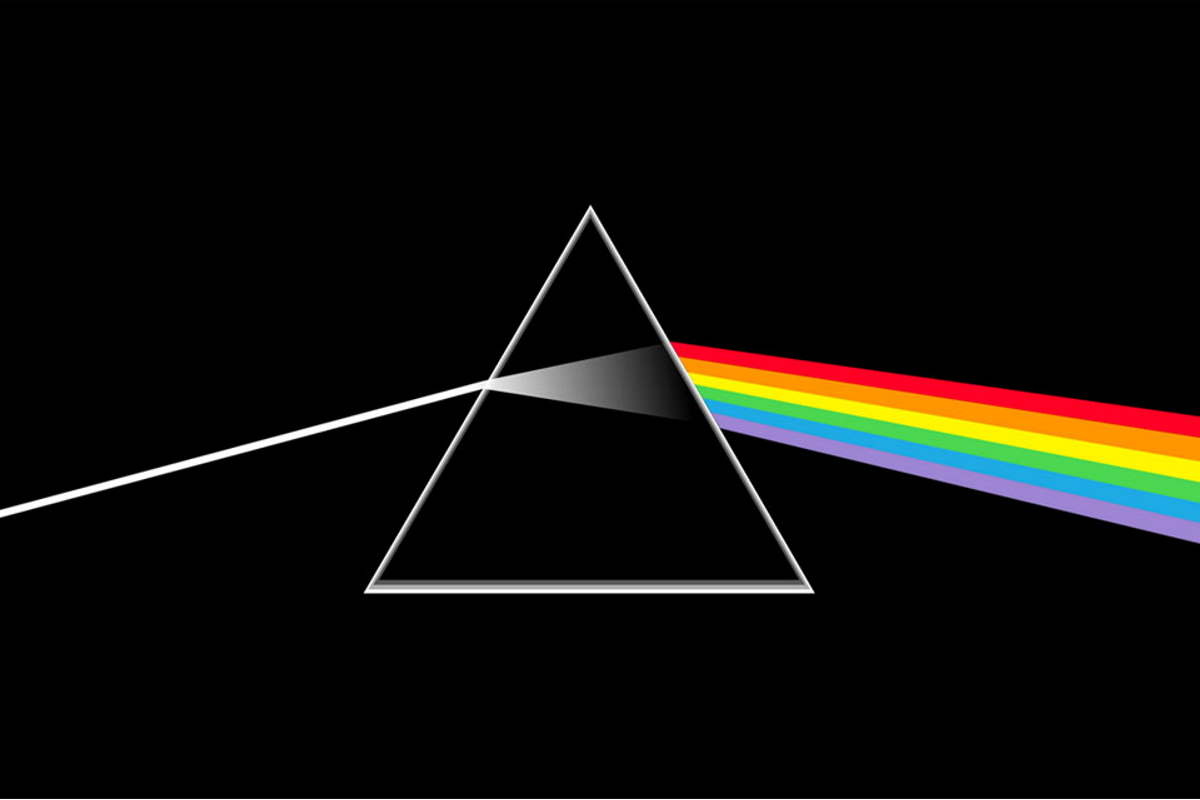
\includegraphics[width=100px]{images/logo.jpg}

\bigskip
\bigskip


\bigskip
{\fontsize{15}{10}\selectfont 
\bigskip


\bigskip
\medskip
{ \textbf{\Huge Moto in un fluido denso \\}}}


\bigskip
\medskip
{ \textbf{ Alberto Mazzarotto}}
\bigskip

\end{center}

\bigskip
\bigskip

\thispagestyle{empty}


\begin{center}
{\Large novembre 2020}
\end{center}


\linespread{1.5}

\newpage\setlength{\parskip}{3mm} 
\onehalfspacing
\bigskip
\pagenumbering{roman}
\setcounter{page}{1}

\begin{center}

{\LARGE \bf Introduzione}

\end{center}
\addcontentsline{toc}{section}{Introduzione}

Come ben sappiamo dalla II legge del caro vecchio Newton \(F=ma\), anche se questa legge è molto comoda per studiare il moto di un corpo a volte non è sufficiente per avere una sua rappresentazione realistica da un punto di vista matematico. Se da un'analisi newtoniana del moto di caduta libera\footnote{Si tratta di un moto uniformemente accelerato.}, usando l'equazione (\ref{eq1}), di una gocciolina di pioggia sembrerebbe che essa possa raggiungere velocità elevatissime sperimentalmente notiamo che non è così: la velocità non supera mai una certa soglia e l'accelerazione non è uniforme.
\begin{equation}\label{eq1}
    s(t)=s_0 + vt + \frac{1}{2}at^2
\end{equation}
Per rappresentare in maniera più accurata il moto di un oggetto attraverso un fluido dobbiamo considerare altri due principi fondamentali: il principio di Archimede, che ci dice che un fluido fornisce una spinta verticale ad un oggetto pari al peso del volume spostato, e la legge di Stokes che ci dice che un oggetto che si muove attraverso un fluido risente di una forza di attrito proporzionale alla sua velocità. Queste due nuove considerazioni sono riassunte nelle seguenti equazioni:
\begin{equation}\label{eq2}
    F_a=-V_{sfera}\;\rho_{fluido}\;\vec g
\end{equation}
\begin{equation}\label{eq3}
    F_s=-b\vec v
\end{equation}
L'analisi di questo tipo di moto verrà fatta in due passaggi; come prima cosa affronterò il problema da un punto di vista puramente teorico e, una volta trovata l'equazione del moto, confronterò i dati empirici misurati in laboratorio con le formule.  
\bigskip


\newpage

\setlength{\parskip}{1mm} 

\tableofcontents
\listoffigures


\newpage \setlength{\parskip}{3mm}
\phantom{ss}
\vspace{-2.5cm}
\sectionfont{\centering}

\renewcommand{\thesection}{\arabic{section}.}

\pagenumbering{arabic}
\setcounter{page}{1}

\section{PARTE TEORICA}
\subsection{Cenni preliminari}
La situazione che prendiamo in considerazione è la seguente: una sfera di cui ci è noto diametro e densità si muove all'interno di un fluido con densità conosciuta. Calcolare la velocità \(v\) a cui si muove la sfera nel generico istante di tempo \(t\). Supponiamo che nell'istante \(t_0 = 0\) la pallina si muova con velocità \(v_0\).
\hfill 

\begin{flushleft}
\textbf{Nomenclatura preliminare}
\end{flushleft}
\begin{center}
\begin{tabular}{ | m{5em} | m{1.4cm}| m{10em} | } 
\hline
variabile &  u.d.m. & descrizione \\ 
\hline
\hline
\(\phi_{sfera}\) & m & diametro sfera \\ 
\hline
\(\rho_{sfera}\) & \(kg/m^3\) & densità sfera \\ 
\hline
\(V\) & \(m^3\) & volume sfera \\ 
\hline
\(m\) & \(kg\) & massa sfera \\ 
\hline
\(\rho_{fluido}\) & \(kg/m^3\) & densità fluido \\ 
\hline
\(F_p\) & \(N\) & forza peso \\ 
\hline
\(F_{pf}\) & \(N\) & forza peso nel fluido \\ 
\hline
\(F_a\) & \(N\) & forza di Archimede \\ 
\hline
\(F_s\) & \(N\) & attrito di Stokes \\ 
\hline
\(g\) & \(m/s^2\) & accelerazione gravità \\ 
\hline
\(b\) & \(kg/s\) & coefficiente di attrito \\ 
\hline
\end{tabular}
\end{center}

\begin{flushleft}
\textbf{Peso di un oggetto in un fluido}\\
Usando Newton e il principio di Archimede posso ricavare il peso di un corpo in un fluido.
\end{flushleft}
\begin{equation}\label{eq4}
    \begin{split}
    F_{pf} &= mg - V\rho_{fluido}\;g\\
        &= V\rho_{corpo}g - V\rho_{fluido}\;g\\
        &=Vg(\rho_{sfera} - \rho_{fluido})
    \end{split}
\end{equation}

\subsection{Analisi}
Partiamo con il trovare la risultante delle forze che agiscono sulla nostra sfera che sono forza peso, spinta di Archimede e attrito esercitato dal fluido.
\begin{equation}\label{eq5}
\vec{R} = \vec{F_p} + \vec{F_a} + \vec{F_s}
\end{equation}
Essendo il moto mono-direzionale assegno alla direzione di \(g\) verso positivo\footnote{La direzione verso il basso per intenderci.}. Sostituisco nell'equazione (\ref{eq4}) la (\ref{eq2}) e la (\ref{eq3}) tenendo conto dei versi dei vettori.
\begin{equation}\label{eq6}
    \begin{split}
    R &= F_p - F_a - F_s\\
            &= mg - V\rho_{fluido}\;g -bv
    \end{split}
\end{equation}
Ricordandoci che \(m=V\rho_{sfera}\) e che, per la II legge di Newton \(R = ma\), risolvo l'equazione per a. Uso anche l'equazione (\ref{eq4}).
\begin{equation}\label{eq7}
    \begin{split}
    ma  &= mg - V\rho_{fluido}\;g -bv\\
        &= V\rho_{sfera}\;g - V\rho_{fluido}\;g -bv\\   
        &= Vg(\rho_{sfera} - \rho_{fluido}) -bv\\
        &= F_{pf} - bv\\
    a   &= \frac{F_{pf} - bv}{m}\\
    a   &=\frac{b}{m}\left(\frac{F_{pf}}{b} - v\right)
    \end{split}
\end{equation}
Possiamo notare ora che \([\frac{b}{m}] = \frac{1}{s}\), è dunque una frequenza che chiamo \(\frac{1}{\mathcal{T}}\), e che \([\frac{F_{pf}}{b}] = \frac{m}{s}\) è quindi una velocità che chiamo \(v_l\). Riscrivendo l'equazione (\ref{eq7}) tenendo conto della nuova nomenclatura ottengo una formula molto carina:
\begin{equation}\label{eq8}
    a = \frac{1}{\mathcal{T}}\left(v_l - v\right)
\end{equation}
Ma \(a\) non è altro che la derivata di \(v\) rispetto al tempo, mi trovo dunque di fronte ad un equazione differenziale che sono in grado di risolvere usando gli integrali.
\begin{equation}\label{eq9}
    \begin{split}
    a = \frac{1}{\mathcal{T}}\left(v_l - v\right)\\
    \frac{a}{v_l - v} = \frac{1}{\mathcal{T}}\\
    \int\frac{a}{v_l - v}\,dt  = \int\frac{1}{\mathcal{T}}\,dt\\
    \int\frac{dv}{v_l - v}\,\frac{dt}{dt}  = \int\frac{1}{\mathcal{T}}\,dt\\
    -\log\lvert v_l - v \rvert = \frac{1}{\mathcal{T}}t + C\\
    \log\lvert v_l - v \rvert = -\frac{1}{\mathcal{T}}t + C
    \end{split}
\end{equation}
Supponendo ora che \(v < v_l\) possiamo togliere il valore assoluto e applicare l'esponenziale.
\begin{equation}\label{eq10}
    \begin{split}
    \log(v_l - v) = -\frac{1}{\mathcal{T}}t\\
    v_l - v = e^{-\frac{1}{\mathcal{T}}t + C}\\
    v = v_l - e^{-\frac{1}{\mathcal{T}}t}e^C\\
    v(t) = v_l - C'e^{-\frac{1}{\mathcal{T}}t}\\
    \end{split}
\end{equation}
Abbiamo finalmente ricavato l'equazione della velocità, per trovare \(C'\) dobbiamo utilizzare le condizioni iniziali che si trovano nei cenni preliminari all'inizio di questo capitolo.
\begin{equation}\label{eq11}
    \begin{cases}
    v_0 = v_l - C'\\
    C' = v_0 - v_l
    \end{cases} \Rightarrow v(t) \; \;= v_l - (v_0 - v_l)e^{-\frac{1}{\mathcal{T}}t}
\end{equation}
Se \(v_0 = 0\) trovo la seguente formula e ho finito:
\begin{equation}\label{eq12}
    \begin{split}
    v(t) &= v_l - v_l e^{-\frac{1}{\mathcal{T}}t}\\
         &= v_l (1 -  e^{-\frac{1}{\mathcal{T}}t})
    \end{split}
\end{equation}


\newpage

\section{PARTE PRATICA}
\subsection{Materiali e descrizione}
L'esperimento consiste nel lasciar cadere una sferetta, in questo caso di metallo, all'interno di un fluido e annotare coppie di valori empirici velocità-tempo confrontandoli con quelli teorici ricavati dalla formula trovata nella sezione precedente. Sinceramente non sono molto soddisfatto degli esperimenti fatti perché il tempo di caduta è troppo breve e questo causa un errore grossolano sia sul rilevamento dei tempi che sull'affidabilità dei valori. Il problema è dovuto al fatto che avrei dovuto scegliere una sferetta di raggio minore (ma non ne avevo in casa), questo perché l'attrito del fluido non è solo proporzionale alla velocità della sfera, ma anche al suo raggio; la legge di Stokes completa per una sfera è infatti:
\begin{equation}
    F_s = - 6\pi\mu rv
\end{equation}
mentre la sua forza antagonista, \(F_pf\) è proporzionale al volume che va come \(r^3\) quindi, per \(r\) grandi, la forza peso vince\footnote{\MakeUppercase{è} simile al rapporto che c'è tra superficie e volume delle cellule: il motivo per cui non abbiamo poche cellule grandi ma tante cellule piccole è che gli scambi chimici avvengono sulla superficie e il rapporto tra superficie e volume non può essere troppo piccolo altrimenti la cellula morirebbe. In una sfera (la nostra cellula) \(V \propto R^3\), mentre \(S \propto R^2\) ne segue che \(S/V \propto 1/R\) e quindi se R cresce troppo la cellula non ha sufficienti scambi per poter stare in vita.} e la sferetta cade svelta. Per limitare i danni ho fatto le riprese a rallentatore per aumentare la precisione delle misure.

\begin{wrapfigure}{r}{0.35\textwidth} %this figure will be at the right
    \centering
    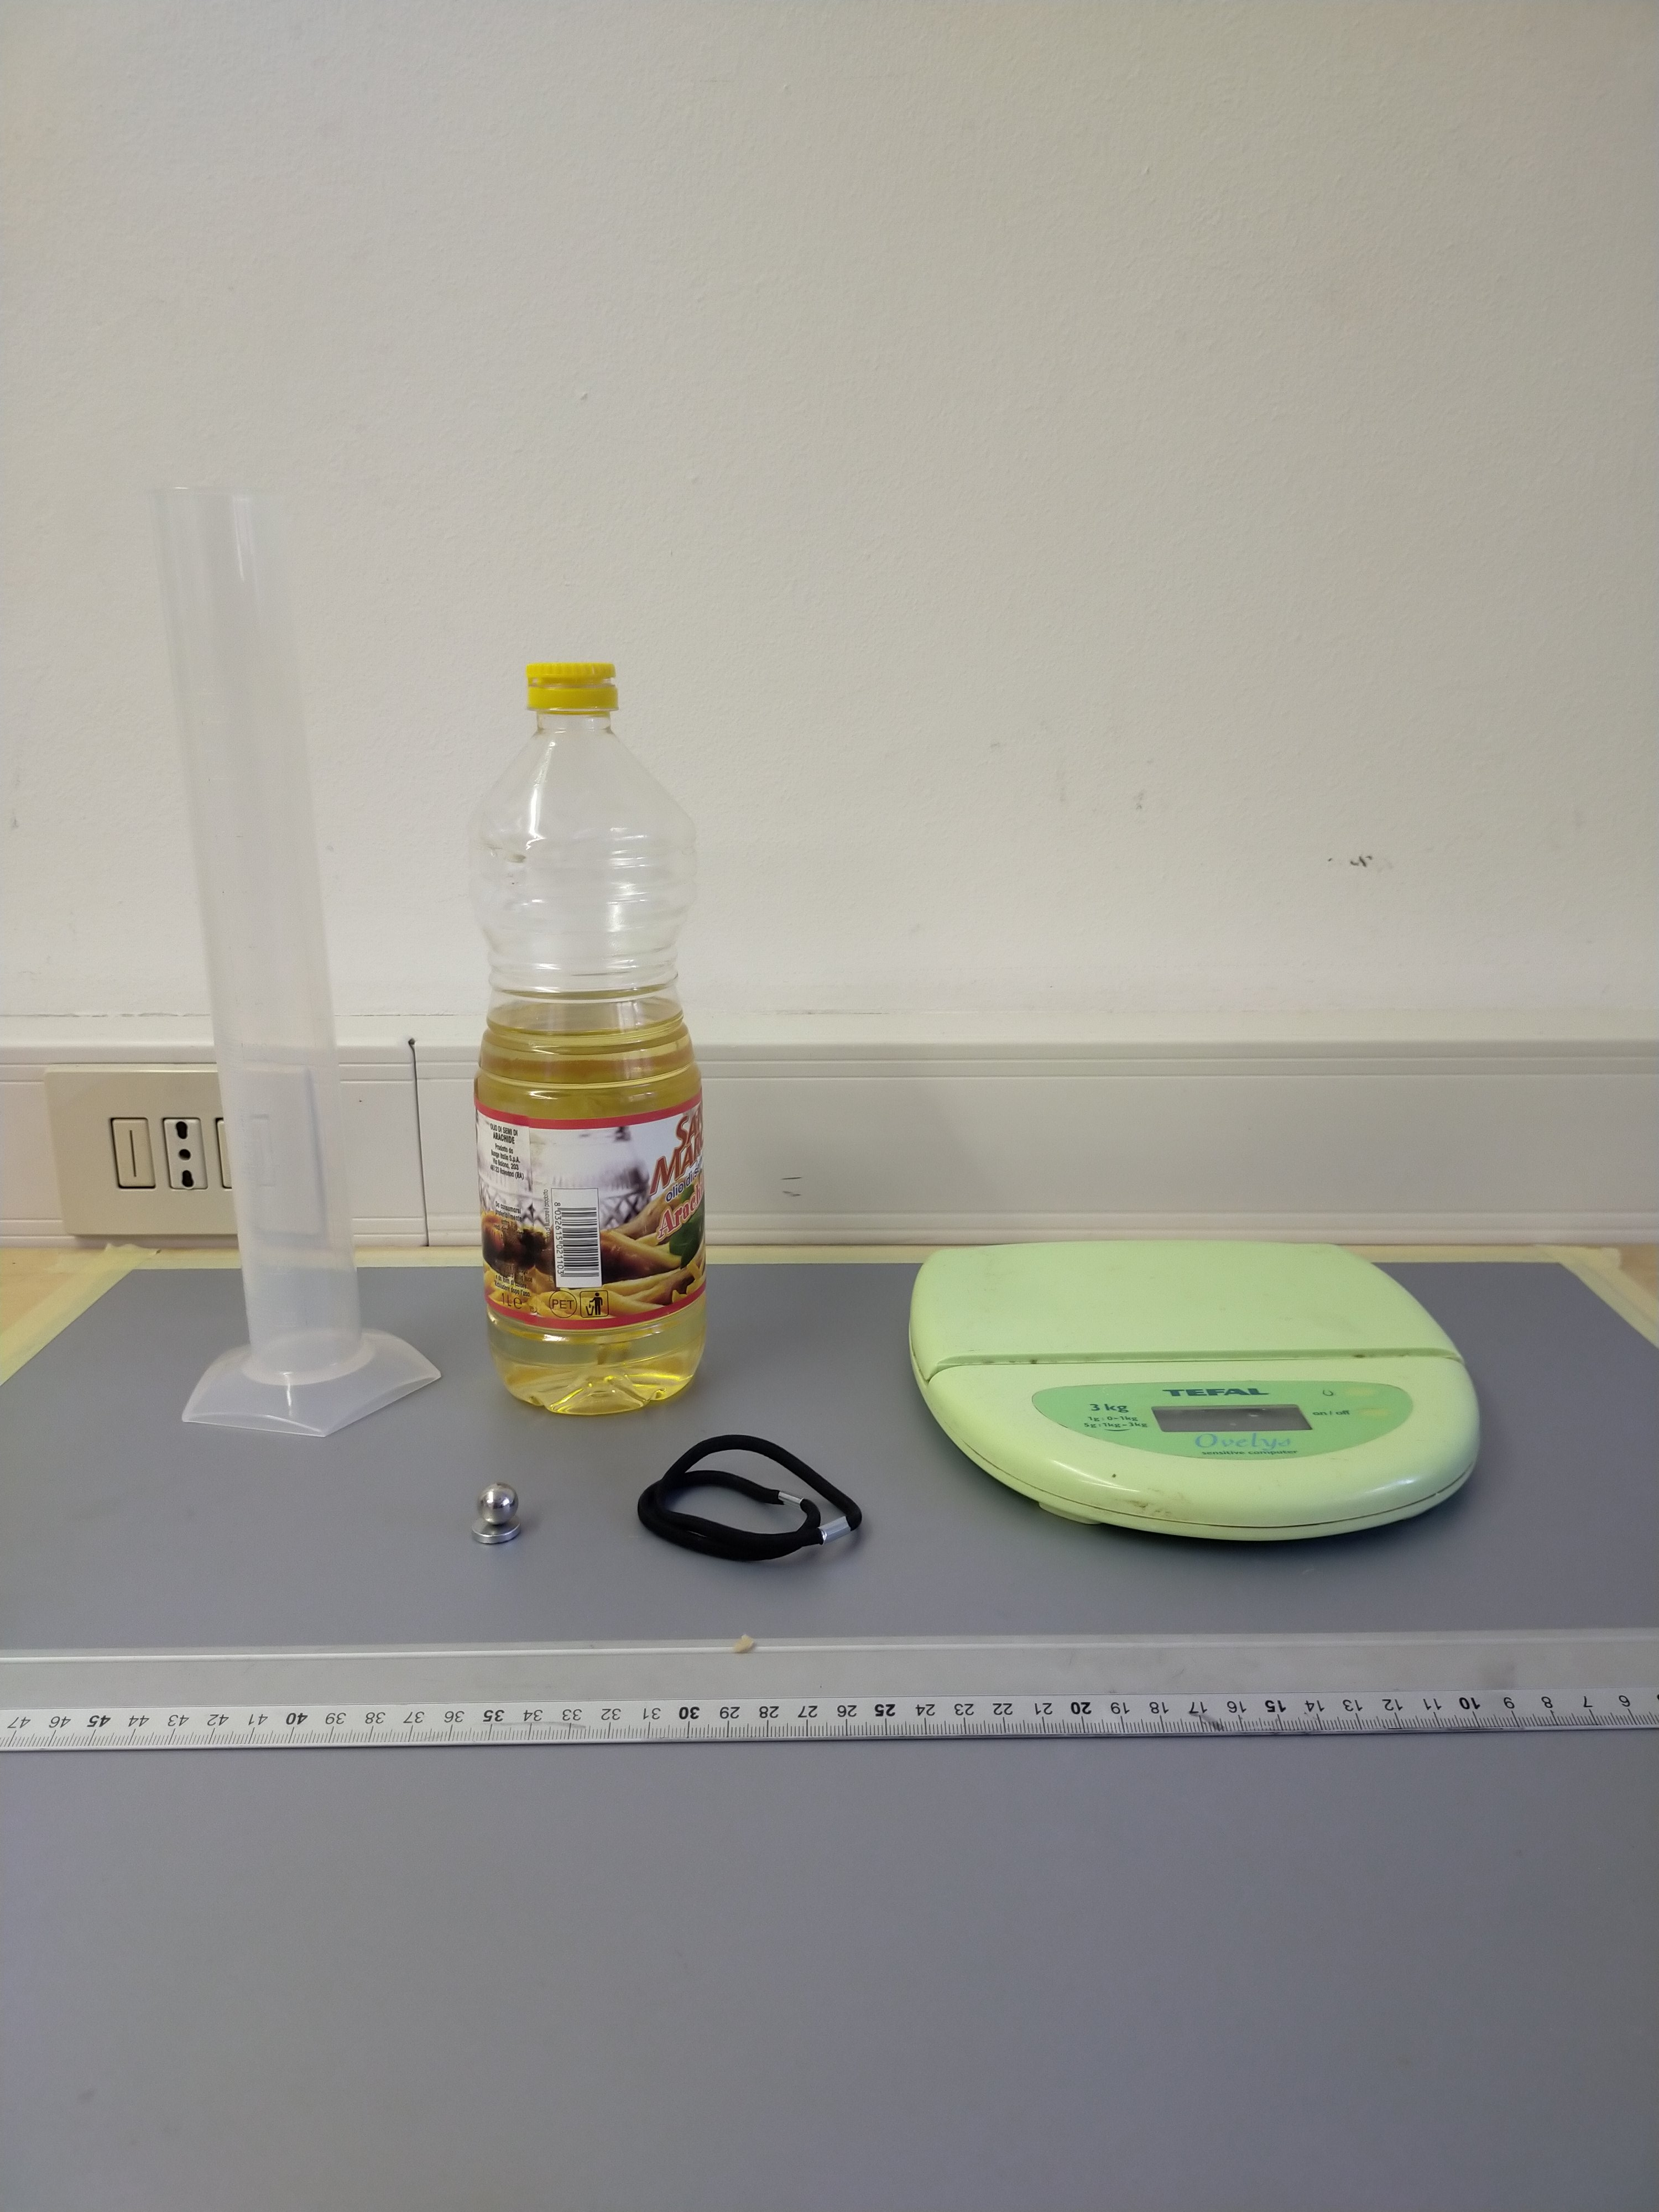
\includegraphics[width=0.35\textwidth]{images/img0.jpg}
    \caption{materiali}
\end{wrapfigure}

\raggedright\textbf{Lista materiali}
\texttt{
\begin{itemize}
    \item Cilindro graduato.
    \item Righello.
    \item Sferetta di metallo.
    \item Olio di semi.
    \item Elastici.
    \item Bilancia.
    \item Magneti (opzionale).
\end{itemize}
}

\clearpage
Un altro problema che ho riscontrato riguarda il timer del telefono che sembra non essere affidabile per quanto riguarda i centesimi di secondo.\\
Per diminuire l'errore sui dati ho deciso, visto gli strumenti digitali a disposizione, di aggiungere alle riprese una barra orrizzontale che ho mappato in modo tale che fosse sempre al centro della mia sfera. 
Supponendo trascurabile la distorsione delle distanze prodotte dall'inclinazione della fotocamera\footnote{Anche se ho avuto cura di posizionare il telefono in modo tale da rendere la normale alla camera più possibile parallela al terreno per limitare questo effetto nulla nella vita è perfetto.} posso utilizzare la posizione in pixel della barra per ricavare una posizione approssimata della sfera nel cilindro. Un ragionamento analogo posso farlo per il tempo: essendo il timer del telefono poco preciso mi affido ai frame del video come unità di misura del tempo. Ovviamente posso poi ricondurmi ad una misura in secondi utilizzando il framerate del video, che è noto, e dando per buoni il $T_{cronometro}$ iniziale e $T_{cronometro}$ finale.
Le equazioni che trasformano $pixel$ in $cm$ e $frame$ in $secondi$ sono le seguenti:
\begin{equation}
s(pxl) = s_0 - \frac{\Delta s}{\Delta pxl}\cdot \delta_{pxl}
\end{equation}
\begin{equation}
t(frame) = t_0 + FPS \cdot \delta_{frame}
\end{equation}
\begin{equation}
\Delta s = \left| s_{finale} - s_{iniziale} \right|
\end{equation}
\begin{equation}
\Delta pxl = \left| pxl_{finale} - pxl_{iniziale} \right|
\end{equation}








\newpage

\section{DATI GREZZI}
\subsection{Dati generali}

\begin{center}
\begin{tabular}{ | m{5em} | m{5em} | m{5em} | m{1.4cm}| m{10em} | } 
\hline
variabile & misura & errore &u.d.m. & descrizione \\ 
\hline
\hline
\(\phi_{sfera}\) & 1.2 & $\pm 1$ & \(cm\) & diametro sfera \\ 
\hline
\(\rho_{sfera}\) & 7800 & & \(kg/m^3\) & densità sfera \\ 
\hline
\(V\)   & 0.90 & & \(m^3\)& volume sfera \\ 
\hline
\(m\) & 8 & $\pm 1$ & \(g\)  & massa sfera \\ 
\hline
\(\rho_{fluido}\) & 908 &  & \(kg/m^3\)& densità fluido \\ 
\hline
\end{tabular}
\end{center}

\newpage
\subsection{Rilevazione 1}

\begin{tabular}{ | m{3em} | m{3em} | m{2.5em}| m{2.5em} | } 
 \hline
 \vspace{5pt} frame \vspace{5pt}  &  pixel & $t(s)$ & $s(cm)$\\ 
 \hline
 \hline
 0 & 493 & 3.52  & 22\\ 
 \hline
 10 & 494 & //  & //\\
 \hline
 20 & 502 & //  & //\\ 
 \hline
 30 & 534 & //  & //\\ 
 \hline
 40 & 582 & //  & //\\ 
 \hline
 50 & 644 & //  & //\\ 
 \hline
 60 & 714 & //  & //\\ 
 \hline
 70 & 794 & //  & //\\ 
 \hline
 80 & 882 & //  & //\\ 
 \hline
 90 & 973 & //  & //\\ 
 \hline
 98 & 1047 & 3.93  & 0.5\\ 
 \hline
\end{tabular}
\quad
\begin{tabular}{ | m{3em} | m{3em} | m{1cm}| } 
 \hline
   &  misura & u.d.m \\ 
 \hline
 \hline
 $\Delta t$   &  0.41 	& s\\
 \hline
 $\Delta s$   &  21.5	& cm\\
 \hline
 $\Delta pxl$ & 554	& pixel\\
 \hline
\end{tabular}



% TABELLA 2%

\newpage
\subsection{Rilevazione 2}

\begin{tabular}{ | m{3em} | m{3em} | m{2.5em}| m{2.5em} | } 
 \hline
 \vspace{5pt} frame \vspace{5pt}  &  pixel & $t(s)$ & $s(cm)$\\ 
 \hline
 \hline
 0 & 488 & 2.41  & 21.3\\ 
 \hline
 10 & 491 & //  & //\\
 \hline
 20 & 507 & //  & //\\ 
 \hline
 30 & 543 & //  & //\\ 
 \hline
 40 & 594 & //  & //\\ 
 \hline
 50 & 656 & //  & //\\ 
 \hline
 60 & 728 & //  & //\\ 
 \hline
 70 & 817 & //  & //\\ 
 \hline
 80 & 906 & //  & //\\ 
 \hline
 90 & 996 & //  & //\\ 
 \hline
 95 & 1041 & 2.82  & 0.5\\ 
 \hline
\end{tabular}
\quad
\begin{tabular}{ | m{3em} | m{3em} | m{1cm}| } 
 \hline
   &  misura & u.d.m \\ 
 \hline
 \hline
 $\Delta t$   &  0.41 	& s\\
 \hline
 $\Delta s$   &  20.8	& cm\\
 \hline
 $\Delta pxl$ & 553	& pixel\\
 \hline
\end{tabular}



% TABELLA 3%

\newpage
\subsection{Rilevazione 3}

\begin{tabular}{ | m{3em} | m{3em} | m{2.5em}| m{2.5em} | } 
 \hline
 \vspace{5pt} frame \vspace{5pt}  &  pixel & $t(s)$ & $s(cm)$\\ 
 \hline
 \hline
 0 & 486 & 2.23  & 22.1\\ 
 \hline
 10 & 493 & //  & //\\
 \hline
 20 & 522 & //  & //\\ 
 \hline
 30 & 564 & //  & //\\ 
 \hline
 40 & 623 & //  & //\\ 
 \hline
 50 & 693 & //  & //\\ 
 \hline
 60 & 769 & //  & //\\ 
 \hline
 70 & 857 & //  & //\\ 
 \hline
 80 & 948 & //  & //\\ 
 \hline
 90 & 1040 & //  & //\\ 
 \hline
 91 & 1041 & 2.61  & 0.5\\ 
 \hline
\end{tabular}
\quad
\begin{tabular}{ | m{3em} | m{3em} | m{1cm}| } 
 \hline
   &  misura & u.d.m \\ 
 \hline
 \hline
 $\Delta t$   &  0.38 	& s\\
 \hline
 $\Delta s$   &  21.6	& cm\\
 \hline
 $\Delta pxl$ & 555	& pixel\\
 \hline
\end{tabular}
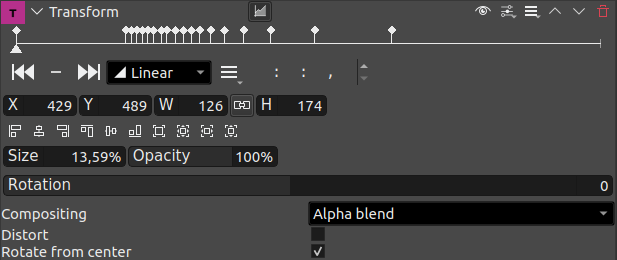
\includegraphics[width=100px]{images/tracking_1.png}

% TABELLA 4 %

\newpage
\subsection{Rilevazione 4}

\begin{tabular}{ | m{3em} | m{3em} | m{2.5em}| m{2.5em} | } 
 \hline
 \vspace{5pt} frame \vspace{5pt}  &  pixel & $t(s)$ & $s(cm)$\\ 
 \hline
 \hline
 0 & 493 & 1.83  & 22\\ 
 \hline
 10 & 497 & //  & //\\
 \hline
 20 & 515 & //  & //\\ 
 \hline
 30 & 549 & //  & //\\ 
 \hline
 40 & 599 & //  & //\\ 
 \hline
 50 & 661 & //  & //\\ 
 \hline
 60 & 734 & //  & //\\ 
 \hline
 70 & 820 & //  & //\\ 
 \hline
 80 & 910 & //  & //\\ 
 \hline
 90 & 1000 & //  & //\\ 
 \hline
 95 & 1045 & 2.23  & 0.2\\ 
 \hline
\end{tabular}
\quad
\begin{tabular}{ | m{3em} | m{3em} | m{1cm}| } 
 \hline
   &  misura & u.d.m \\ 
 \hline
 \hline
 $\Delta t$   &  0.40 	& s\\
 \hline
 $\Delta s$   &  21.8	& cm\\
 \hline
 $\Delta pxl$ & 552	& pixel\\
 \hline
\end{tabular}


% TABELLA 5%

\newpage
\subsection{Rilevazione 5}

\begin{tabular}{ | m{3em} | m{3em} | m{2.5em}| m{2.5em} | } 
 \hline
 \vspace{5pt} frame \vspace{5pt}  &  pixel & $t(s)$ & $s(cm)$\\ 
 \hline
 \hline
 0 & 498 & 1.70 & 21.8\\ 
 \hline
 10 & 501 & //  & //\\
 \hline
 20 & 514 & //  & //\\ 
 \hline
 30 & 550 & //  & //\\ 
 \hline
 40 & 596 & //  & //\\ 
 \hline
 50 & 650 & //  & //\\ 
 \hline
 60 & 721 & //  & //\\ 
 \hline
 70 & 805 & //  & //\\ 
 \hline
 80 & 889 & //  & //\\ 
 \hline
 90 & 979 & //  & //\\ 
 \hline
 97 & 1042 & 2.11  & 0.2\\ 
 \hline
\end{tabular}
\quad
\begin{tabular}{ | m{3em} | m{3em} | m{1cm}| } 
 \hline
   &  misura & u.d.m \\ 
 \hline
 \hline
 $\Delta t$   &  0.41 	& s\\
 \hline
 $\Delta s$   &  21.6	& cm\\
 \hline
 $\Delta pxl$ & 544	& pixel\\
 \hline
\end{tabular}


\end{document}
